\documentclass[fleqn,11pt]{article}

% __________________________________________________________ PACKAGES AND DEFINITIONS
% ___________________________________________________________________________________

% Numbering of sections and subsections
\setcounter{secnumdepth}{3}

% This avoids redundancy in math alphabets
\newcommand{\bmmax}{0}

\usepackage[a4paper, total={160mm,240mm}]{geometry}
\usepackage{amsfonts, amsmath, bm}
\usepackage{setspace}
\usepackage{subcaption}
\usepackage[font=footnotesize]{caption}
\captionsetup[table]{skip=0pt}

% tikz
\usepackage{tikz}
\usepackage{pgfplots}
\pgfplotsset{compat=1.17}

% Avoid re-drawing unchanged tikz figures
\usetikzlibrary{external}
\tikzexternalize

% Bibliography style
\bibliographystyle{spmpsci}

% Font
\renewcommand*\rmdefault{bch}

% Spacing
\setstretch{1.5}
\renewcommand{\arraystretch}{1.136}
\setlength{\parskip}{1em}				% Separation between paragraphs
\frenchspacing

% Spacing before section titles
\usepackage{titlesec}
%\titlespacing*{<command>}{<left>}{<before-sep>}{<after-sep>}
\titlespacing*{\section}
{0pt}{8ex plus 1ex minus .2ex}{0.3ex plus .2ex minus .2ex}
\titlespacing*{\subsection}
{0pt}{7ex plus 1ex minus .2ex}{0.3ex plus .2ex minus .2ex}

\setlength{\skip\footins}{1cm}

% Headers
\usepackage{fancyhdr}
\pagestyle{fancy}
\setlength\headheight{26pt}
\renewcommand{\footrulewidth}{0.4pt}% default is 0pt

% This one is needed to avoid two "REFERENCES" header in the bibliography pages
\fancypagestyle{bib}{
	\fancyhf{}
	\fancyhead[LE,RO]{%
		% We want italics
		\itshape
		% The chapter title
		\leftmark}
	\fancyfoot[C]{\thepage}
}


% Empty page at the end of a section
\def\blankpage{%
	\clearpage%
	\thispagestyle{empty}%
	\addtocounter{page}{-1}%
	\null%
	\clearpage}

% ____________________________________________________________________________ MACROS
% ___________________________________________________________________________________

\definecolor{brick_red}			{RGB}{128,0,0}
\definecolor{dark_blue}			{RGB}{75,120,200}
\definecolor{dark_green}		{RGB}{0,128,0}

\definecolor{Blue}				{RGB}{48,39,238}
\definecolor{Red}				{RGB}{230,48,39}
\definecolor{Black}				{RGB}{0,0,0}
\definecolor{Green}				{RGB}{38,128,29}
\definecolor{Orange}			{RGB}{237,125,49}

\definecolor{DarkBlue}			{RGB}{0,0,64}
\definecolor{LightBlue}			{RGB}{120,120,255}
\definecolor{PaleBlue}			{RGB}{200,200,255}

\definecolor{DarkGreen}			{RGB}{0,64,0}
\definecolor{LightGreen}		{RGB}{60,220,60}
\definecolor{PaleGreen}			{RGB}{120,255,120}

% Points
\newcommand{\point}[1]{ \mathsf{ #1 } }
\newcommand{\ptA}		{ {\point{A}}}
\newcommand{\ptB}		{ {\point{B}}}
\newcommand{\ptP}		{ {\point{P}}}
\newcommand{\ptQ}		{ {\point{Q}}}

% Units
\newcommand{\unit}[1]		{ {\; \rm #1} }

% Parentheses
\newcommand{\plbr}[1]{ \left( #1 \right) }
\newcommand{\sqbr}[1]{ \left[ #1 \right] }
\newcommand{\lcubr}[1]{ \left\{ #1 \right.}

% Matrices
\newcommand{\matr}[2]{ \sqbr{\begin{array}{ #1 } #2 \end{array} }}
\newcommand{\matrArray}[2]{ \begin{array}{ #1 } #2 \end{array} }

% Derivatives
\newcommand{\partialD}[2]{ \dfrac{\partial #1}{\partial #2}}
\newcommand{\totalD}[2]{ \dfrac{{\rm d} #1}{{\rm d} #2}}

\newcommand{\trans}		{ ^{\rm T} }
\newcommand{\inv}		{ ^{-1} }
\newcommand{\zero}		{ {\bf 0} }
\newcommand{\eye}		{ {\bf I} }
\newcommand{\eq}		{ {\;=\;} }

\newcommand{\pos}		{ {\bf{q}} }
\newcommand{\vel}		{ {{\dot{\bf{q}}}} }
\newcommand{\acc}		{ {\ddot{\bf{q}}} }
\newcommand{\Mass}		{ {\bf{M}} }
\newcommand{\fCor}		{ {\bf{c}} }
\newcommand{\f}			{ {\bf{f}} }
\newcommand{\fh}		{ {\bf{f}_{\rm h}} }
\newcommand{\Damp}		{ {\bf{C}} }
\newcommand{\Stiff}		{ {\bf{K}} }

\newcommand{\ctr}		{ {\bm \Phi} }
\newcommand{\ctrJac}	{ {\bm \Phi}_{\pos} }
\newcommand{\ctrJacd}	{ {\dot{\bm \Phi}}_{\pos} }
\newcommand{\fgen}		{ {\bf Q} }
\newcommand{\LagMult}	{ {\bm \lambda} }
\newcommand{\Jac}		{ {\bf J} }

\newcommand{\pres}		{ {\bf{p}} }
\newcommand{\presd}		{ {\dot{\bf{p}}} }

% Time-steps
\newcommand{\hM}    	{ h_{\mathcal{M}} }
\newcommand{\hH}     	{ h_{\mathcal{H}} }

% Inputs and outputs
\newcommand{\inputs}  	{ {\bf u} } 
\newcommand{\outputs}  	{ {\bf y} } 
\newcommand{\inputM}  	{ {\bf u}_{\mathcal{M}} }
\newcommand{\outputM}  	{ {\bf y}_{\mathcal{M}} }
\newcommand{\inputH}   	{ {\bf u}_{\mathcal{H}} }
\newcommand{\outputH}  	{ {\bf y}_{\mathcal{H}} }


% ___________________________________________________________________________________
% ___________________________________________________________________________________

\begin{document}
	
\vspace{1cm}

\title{\LARGE \bf Co-simulation benchmarks: 2-d.o.f hydraulic manipulator}

\author{\\ \bf Laboratorio de Ingenier\'ia Mec\'anica - LIM \\ \bf Universidade da Coru\~na}

\maketitle

{\let\newpage\relax\maketitle}
{\thispagestyle{fancy}
	\fancyfoot[C]{}
	\lhead{
\includegraphics[width=1.24cm]{./fig/LIM-logo.pdf}}
	\rhead{
\includegraphics[width=3.4cm]{./fig/cosimbauto-logo.pdf}}}

\newpage

\fancyhf{}
\pagestyle{fancy}
\fancyhead[L]{\ifodd\value{page}\else
	Planar hydraulic manipulator \fi}
\fancyhead[C]{\ifodd\value{page} \fi}
\fancyhead[R]{\ifodd\value{page} Benchmark problem \fi}
\fancyfoot[C]{\thepage}
	
	
% ___________________________________________________________________________________

\textit{
	This document describes a benchmark problem for the co-simulation of mechanical and hydraulic systems in multirate schemes.
	A general overview of the assembly is provided, together with a reference implementation of the dynamics equations of both subsystems.
	Moreover, simulation results are provided as reference for selected solution methods of the co-simulation equations.
	These can be used to validate simulation results obtained with new implementations of the same model.
}


% ___________________________________________________________________________________
\section{Problem description}
\label{ProblemDefinition}

A planar model of a hydraulically actuated two-link robotic arm is shown in Fig.~\ref{fig:crane}.
A similar model was described in \cite{Naya2011} and used as benchmark problem in \cite{Peiret2018}.

\begin{figure}[htbp]
	\centering
	\begin{tikzpicture}
		\useasboundingbox (-6cm,-3cm) rectangle (6cm,3cm);
		
		% Figure Drawing
		\node at (0,0) {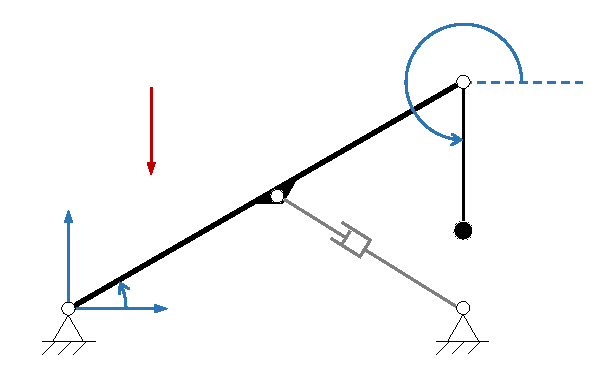
\includegraphics[width=0.53\textwidth]{./fig/craneNoLabels.pdf}};
		
		% Text
		\coordinate (nodeLink1) at (-25mm, -5mm);  	
		\node[anchor=east] at (nodeLink1) {{\color{black}$1$}};
		\draw (nodeLink1) to[out=0,in=120] ++(6mm,-4mm);
		
		\coordinate (nodeLink2) at (34mm, -1mm);  
		\node[anchor=west] at (nodeLink2) {{\color{black}$2$} {\footnotesize (massless)}};
		\draw (nodeLink2) to[out=180,in=0] ++(-8mm,-3mm);
		
		\coordinate (nodeX) at (-20mm, -21.75mm);       \node at (nodeX) {{\color{dark_blue}$x$}};
		\coordinate (nodeY) at (-37.75mm, -5.75mm);     \node at (nodeY) {{\color{dark_blue}$y$}};
		\coordinate (nodeTh1) at (-21.75mm, -15.9mm);   \node at (nodeTh1) {{\color{dark_blue}$\theta_1$}};
		\coordinate (nodeTh2) at (35.75mm, 21.75mm);    \node at (nodeTh2) {{\color{dark_blue}$\theta_2$}};
		
		\coordinate (nodeG) at (-18.5mm, 8.5mm);        \node at (nodeG) {{\color{brick_red}$g$}};
		
		\coordinate (node1) at (-5.5mm, 1.5mm);         \node at (node1) {{\color{black}$\point{P}$}};
		\coordinate (node2) at ( 28.7mm, 12.1mm);       \node at (node2) {{\color{black}$\point{Q}$}};
		\coordinate (node3) at ( 28.7mm, -10mm);        \node at (node3) {{\color{black}$\point{R}$}};
		\coordinate (nodeA) at ( -38mm, -18mm);         \node at (nodeA) {{\color{black}$\point{O}$}};
		\coordinate (nodeB) at ( 28.5mm, -18mm);        \node at (nodeB) {{\color{black}$\point{B}$}};
		
		\coordinate (nodeL) at ( 5mm, 8mm);             \node at (nodeL) {{\color{black}$L$}};
		\coordinate (nodeLh) at ( 28.5mm, 3mm);         \node at (nodeLh) {{\color{black}$L_{\text{h}}$}};
		\coordinate (nodeS1) at ( 5mm, -12mm);          \node at (nodeS1) {{\color{black}$s_1$}};
		
	\end{tikzpicture}
	\caption{Planar model of a manipulator with a single hydraulic actuator}
	\label{fig:crane}
\end{figure}

This hydraulically actuated mechanical system can be used as benchmark for multirate co-simulation schemes.
Many different implementation approaches can be used to represent its components.
Here, we will be using as reference implementation a minimal coordinates representation to describe the two-link pendulum, and the first order ordinary differential equations used to formulate the hydraulics in \cite{Naya2011}. 

% ____________________________________________
\subsection{Multibody model}
\label{MultibodyModel}

Link 1 is a rod of length $L$ and distributed mass $m$.
Link 2 has length $L_{\text{h}}$ and is considered to be massless.
Two point masses $m_{\text{p}}$ and $m_{\text{h}}$ are placed at points $\point{Q}$ and $\point{R}$.
The system moves under gravity effects (gravity acts along the negative direction of the $y$ axis) and is actuated with a hydraulic piston that connects points $\point{B}$~and~$\point{P}$.
The length of the actuator is denoted by variable $s_1$.
The values of the system properties used in the numerical experiments are summarized in Table \ref{tab:crane_parameters}.

\begin{table}[htbp]
\begin{center}
{
	\renewcommand{\arraystretch}{1.25}
	\begin{tabular}{lc@{\qquad}r}
		\hline
		Length of link 1     	 				& $L$                     & 1.0~m  \\
		Length of link 2 						& $L_{\text{h}}$          & 0.5~m  \\
		Mass of link 1                          & $m$                     & 200~kg \\
		Point mass at $\point{Q}$               & $m_{\text{p}}$          & 250~kg \\
		Point mass at $\point{R}$               & $m_{\text{h}}$          & 100~kg \\
		Coordinates of fixed point $\point{B}$  & $\plbr{x_{\point{B}},y_{\point{B}}}$  & $\plbr{\sqrt{3}/2, 0}$~m \\
		Initial angle, link 1                   & $\plbr{\theta_1}_0$     & $\pi/6$~rad \\
		Initial angle, link 2                   & $\plbr{\theta_2}_0$     & $3\pi/2$~rad \\
		Gravity                                 & $g$                     & $-9.81$~m/s$^2$ \\
		\hline
	\end{tabular}
}
\end{center}
\caption{Mechanical parameters of the single-actuated model}
\label{tab:crane_parameters}
\end{table}

The system is modelled using a set of minimal coordinates $\pos = \sqbr{\theta_1,\theta_2}\trans$, where $\theta_1$ and $\theta_2$ are the angles from the $x$-axis to rods 1 and 2, as shown in Fig.~\ref{fig:crane}.
The dynamics equations in independent coordinates can be given as
\begin{equation}
	\Mass\acc + \fCor = \f + \fh
	\label{eq:MBSDynamics}
\end{equation}
where $\Mass$ is the mass matrix, $\fCor$ contains the velocity-dependent forces and Coriolis terms, $\fh$ represents the force applied by the hydraulic piston, and $\f$ stands for every other applied force in the system.
In this example, the terms in Eq.~\eqref{eq:MBSDynamics} take the form
\begin{align}
	\Mass &= \matr{cc}{
		\dfrac{L^2 \plbr{m+m_{\text{p}}+m_{\text{h}}}}{3} & LL_{\text{h}} m_{\text{h}} \cos\plbr{\theta_1-\theta_2} \\
		LL_{\text{h}} m_{\text{h}} \cos\plbr{\theta_1-\theta_2} & L_{\text{h}}^2 m_{\text{h}}
	}\;,
	\notag \\[2mm]
	\fCor &= LL_{\text{h}} m_{\text{h}} \sin\plbr{\theta_1 - \theta_2} 
	\matr{c}{\dot{\theta}_2^2 \\ -\dot{\theta}_1^2}
	\;, \quad\quad
	\f = \matr{c}{ 
		- \dfrac{Lg}{2}\plbr{m + m_{\text{p}} + m_{\text{h}}}\cos{\theta_1} \\
		- L_{\text{h}}gm_{\text{h}}\cos{\theta_2}
	}
\label{eq:MBSDynamicsExpr}
\end{align}
The force exerted by the hydraulic piston on the two-link pendulum, expressed in the generalized coordinates $\pos$, can be computed by means of
\begin{equation}
	\fh = \Jac\trans f_{\text{h}}
	\label{eq:HydroForce}
\end{equation}
where $f_{\text{h}}$ is the magnitude of the force exerted by the actuator and $\Jac$ is the velocity transformation matrix that relates the generalized velocities of the multibody system, $\vel$, and the actuator rate, $\dot{s}_1$, \cite{Kovecses2008}
\begin{equation}
	\dot{s}_1 = \Jac \vel
	\label{eq:velTransf}
\end{equation}
For the dimensions in Table~\ref{tab:crane_parameters}, and for any position of the mechanism,
\begin{equation}
	s_1 = L\, \sqrt{ 1 - \dfrac{\sqrt{3}}{2}\cos{\theta_1}} \;, \quad\quad\quad\quad  
	\Jac = \matr{cc}{\dfrac{\sqrt{3}L^2\sin{\theta_1}}{4s_1} &0}
	\label{eq:actLength}
\end{equation}

The system accelerations $\acc$ can be directly evaluated from Eq.~\eqref{eq:MBSDynamics} and integrated using numerical methods to obtain the time evolution of the mechanism.
The reference integration method used in this document is the semi-implicit forward Euler formula, which represents a good trade-off between simplicity and accuracy \cite{Gonzalez2016}
\begin{align}
	\vel_{k+1} &= \vel_k + h \acc_k
	\\
	\pos_{k+1} &= \pos_k + h \vel_{k+1}
	\label{eq:sifwE}
\end{align}
where subscript $k$ denotes the time-step, and $h$ is the integration step-size.


% ____________________________________________
\subsection{Hydraulic model}
\label{HydraulicModel}

The dynamics of the hydraulic system was evaluated using the hydraulic model in \cite{Naya2011}.
The hydraulics is described by a set of first order ordinary differential equations (ODE) in which the system pressures are the integration variables.
The magnitude of the hydraulic force exerted by the actuator can be evaluated as
\begin{equation}
	f_{\text{h}} = \left( p_2 - p_1 \right) a_\text{p} - c \dot{s}_1
	\label{eq:hydForce}
\end{equation}
where $p_1$ and $p_2$ are the fluid pressures within the cylinder, as shown in Fig.~\ref{fig:cylinder} and $a_\text{p}$ is the total piston area.
A viscous friction model with coefficient $c$ was used to represent internal dissipation in the actuator.
We group pressures $p_1$ and $p_2$ in term $\pres = \sqbr{p_1, p_2}\trans$.

\begin{figure}[ht]
	\centering
	\begin{tikzpicture}
		
		% Figure Drawing
		\node at (0,0) {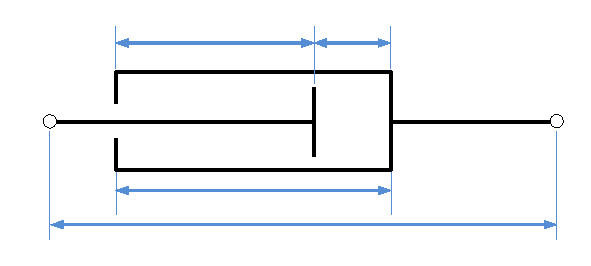
\includegraphics[width=0.55\textwidth]{./fig/cylinderNoLabels.pdf}};
		
		% Text total length
		\node at (1mm, -17mm) {{\color{dark_blue}$s_1$}};
		
		% Other lengths
		\node at (-8mm, -11.5mm) {{\color{dark_blue}$l$}};
		\node at (-12mm, 17mm) {{\color{dark_blue}$l_1$}};
		\node at (9mm, 17mm){{\color{dark_blue}$l_2$}};
		
		% Pressures
		\node at (-18mm, 5mm) {{\color{dark_green}$p_1$}};
		\node at (8mm, 5mm) {{\color{dark_green}$p_2$}};
		
	\end{tikzpicture}
	\caption{Schematic of the hydraulic actuator}
	\label{fig:cylinder}
\end{figure}

The dynamics of the hydraulic system can be described with the following set of first order ODEs \cite{Naya2011}
\begin{align}
	\label{eq:hydODE1}
	\dot{p}_1 
	&= 
	\dfrac{\beta_1}{a_\text{p} l_1}
	\sqbr{a_\text{p} \dot{s}_1 
		+ a_{\text{i}} c_{\text{d}} \sqrt{\dfrac{2 \plbr{p_{\text{P}} - p_1}}{\rho}}\delta_{\text{P1}} 
		- a_{\text{o}} c_{\text{d}} \sqrt{\dfrac{2 \plbr{p_1 - p_{\text{T}}}}{\rho}}\delta_{\text{T1}}}
	\\[2mm]
	\dot{p}_2 
	&= 
	\dfrac{\beta_2}{a_\text{p} l_2}
	\sqbr{- a_\text{p} \dot{s}_1 
		+ a_{\text{o}} c_{\text{d}} \sqrt{\dfrac{2 \plbr{p_{\text{P}} - p_2}}{\rho}}\delta_{\text{P2}} 
		- a_{\text{i}} c_{\text{d}} \sqrt{\dfrac{2 \plbr{p_2 - p_{\text{T}}}}{\rho}}\delta_{\text{T2}}}
	\label{eq:hydODE2}
\end{align}
where $l_1$ and $l_2$ are the variable lengths of the chambers on each side of the piston, $a_{\text{i}}$ and $a_{\text{o}}$ are the variable valve areas that connect these cylinder chambers to the pump and the tank in the hydraulics system, $c_{\text{d}}$ is the discharge coefficient of the valves, $\rho$ stands for the fluid density, $p_{\text{P}}$ and $p_{\text{T}}$ are the hydraulic pressure at the pump and the tank respectively. 
Coefficients $\delta_{\text{P1}}$, $\delta_{\text{P2}}$, $\delta_{\text{T1}}$, and $\delta_{\text{T2}}$ are 0 when the quantity inside the square root that precedes them is negative and 1 otherwise.
Terms $\beta_1$ and $\beta_2$ stand for the bulk modulus in each cylinder chamber, and they are evaluated as a function of the fluid pressure \cite{Cardona1990}
\begin{equation}
	\beta_i = \dfrac{1+ap_i+bp_i^2}{a+2bp_i}\,, \quad i=1,2
	\label{eq:bulkModulus}
\end{equation}
where $a$ and $b$ are constants for the fluid.
Assuming that the two cylinder chambers have equal volume at the starting time of the simulation, chamber lengths $l_1$ and $l_2$ are given by
\begin{equation}
	\begin{split}
		l_1 = 0.5 l + s_{1,0} - s_1
		\\
		l_2 = 0.5 l + s_1 - s_{1,0}
	\end{split}
	\label{eq:chamberLengths}
\end{equation}
where $s_{1,0}$ is the initial length of the actuator.
Valve areas $a_{\text{i}}$ and $a_{\text{o}}$ have m$^2$ units and are obtained as
\begin{equation}
	\begin{aligned}
		a_{\text{i}} &= 5 \cdot 10^{-4} \kappa
		\\
		a_{\text{o}} &= 5 \cdot 10^{-4} \plbr{1-\kappa}
	\end{aligned}
	\label{eq:ValveAreas}
\end{equation}
In Eq.~\eqref{eq:ValveAreas}, $\kappa \in \sqbr{0,1}$ is the valve control parameter or spool displacement, i.e., the kinematic input that controls the motion of the piston.
The hydraulic subsystem parameters for this problem are shown in Table \ref{tab:hydrParams}.

\begin{table}[ht]
\begin{center}
{
	\renewcommand{\arraystretch}{1.25}
	\begin{tabular}{lcr}
		\hline
		Piston area                        & $a_\text{p}$      & $65 \cdot 10^{-4}$ m$^2$       \\
		Cylinder length                    & $l$               & $0.442$ m                      \\
		Friction coefficient               & $c$               & $10^5$ Ns/m                    \\
		Valve discharge coefficient        & $c_{\text{d}}$    & $0.67$                         \\
		Fluid density                      & $\rho$            & $850$ kg/m$^3$                 \\
		Hydraulic pressure at the pump     & $p_{\text{P}}$    & $7.6$ MPa                      \\
		Hydraulic pressure at the tank     & $p_{\text{T}}$    & $0.1$ MPa                      \\
		Compressibility coefficient        & $a$               & $6.53 \cdot 10^{-10}$ Pa       \\
		Compressibility coefficient        & $b$               & $-1.19 \cdot 10^{-18}$         \\
		\hline
	\end{tabular}
}
\end{center}
\caption{Hydraulic parameters}
\label{tab:hydrParams}
\end{table}

The dynamics of the hydraulics system is integrated using a forward Euler formula as well.
Because Eqs.~\eqref{eq:hydODE1} and \eqref{eq:hydODE2} are first-order ODEs, a single integration formula is necessary
\begin{equation}
	\pres_{k+1} = \pres_k + h\presd_k
	\label{eq:fwE}
\end{equation}
where again $k$ stands for the time-step and $h$ for the integration step-size.


% ____________________________________________
\subsection{Initial equilibrium configuration}
\label{InitialEquilibrium}

It is necessary to make sure that the system is initially in a state of static equilibrium.
The simulation must start from a stable initial configuration, to guarantee the correctness of the obtained results.
Ideally, this should result in the satisfaction of the following conditions
\begin{itemize}
	\item{ The initial accelerations $\acc$ and velocities $\vel$ of the multibody system are zero.}
	\item{ The rates of change of the hydraulic pressures with respect to time, $\presd$, are zero as well.}
	\item{ The force $f_{\text{h}}$ exerted by the hydraulic piston balances the weight of the mechanical system.} 
\end{itemize}

\vspace{0.5cm}
The following procedure can be used to determine the initial static equilibrium configuration.
These steps must be performed before the start of the time integration of the system dynamics.
\begin{enumerate}
	\item{
		The multibody system can be initialized setting $\pos = \sqbr{\plbr{\theta_1}_0,\plbr{\theta_2}_0}\trans$ and $\vel = \zero$.
	} 
	\item{
		For these values of the system generalized positions and velocities, the hydraulic force required to keep the static equilibrium of the mechanical system can be evaluated as \cite{Peiret2018}
		\begin{equation}
			f_{\text{h}} = -\Mass_{\text{eff}} \, \Jac \, \Mass\inv \plbr{\f-\fCor}\,
			\quad\quad\quad
			{\text{where }} \Mass_{\text{eff}} = \plbr{\Jac \Mass\inv \Jac\trans}\inv
			\label{eq:effectiveForce}
		\end{equation}
	}
	\item{
		The actuator length $s_1$ and rate $\dot{s}_1$ can be evaluated using Eqs.~\eqref{eq:velTransf} and \eqref{eq:actLength}.
	}
	\item{
		Once they are known, the initial values of $s_1$, $\dot{s}_1$, and $f_{\text{h}}$ must be used to determine the initial state of the hydraulics subsystem.
		An iterative algorithm, which requires an initial guess of the system pressures $\pres$ and the valve control parameter $\kappa$, must be used because of the nonlinearity of differential equations \eqref{eq:hydODE1} and \eqref{eq:hydODE2}.
		A possibility is using a Newton-Raphson scheme, in which pressures $\pres$ and the actuation $\kappa$ are updated according to
		\begin{equation}
			{\bf z}^{i+1} = {\bf z}^{i} + \Delta{\bf z}^{i}  
			\quad \quad \quad \text{where } {\bf z} = \sqbr{p_1, p_2, \kappa}\trans
			\quad \text{ and }
			\Delta{\bf z} = - \totalD{\bf g}{\bf z}\, {\bf g}
			\label{eq:NRiniHyd}
		\end{equation}
		where superscript $i$ stands for the iteration number.
		Function $\bf g$ in Eq.~\eqref{eq:NRiniHyd} represents the initial equilibrium conditions, given by Eqs.~\eqref{eq:hydForce}, \eqref{eq:hydODE1}, and \eqref{eq:hydODE2}
		\begin{equation}
			{\bf g} = \matr{c}{
				f_{\text{h}} - \plbr{p_2-p_1}a_{\text{p}} \\ \dot{p}_1 \\ \dot{p}_2
			} = \zero
			\label{eq:residual}
		\end{equation} 
		The iteration can be performed until the norm of the residual in Eq.~\eqref{eq:residual} falls below a certain maximum admissible value, or until a fixed number of iterations is completed.
		Upon convergence of the iterative procedure, the initial values of $\pres$, $\presd$, and $\kappa$ are obtained.
	}
\end{enumerate}

\vspace{0.5cm}
For the system parameters and initial configuration referred in Sections \ref{MultibodyModel} and \ref{HydraulicModel}, the initial hydraulic force is $f_{\text{h}} = 8.829\unit{kN}$ and the actuator length is $s_1 = 0.5\unit{m}$.
Initializing the hydraulics with these values and performing three iterations of the Newton-Raphson procedure in Eq.~\eqref{eq:NRiniHyd}, this results in the following initial values for the hydraulics
\begin{equation}
	p_1 = 3.1708\unit{MPa}\;, \quad\quad p_2 = 4.5292\unit{MPa}\;, \quad\quad \kappa_0 = 0.4543
	\label{eq:iniValHyd}
\end{equation}
where $p_1=3.3\unit{MPa}$, $p_2=4.4\unit{MPa}$, $\kappa = 0.5$ were used as initial guess.


% _______________________________________________________________________________________________
\newpage
\section{Manoeuvres}
\label{Manoeuvres}

Two manoeuvres were defined to evaluate the behaviour of co-simulation schemes with this benchmark example.
The first one consisted in a two-step variation of the valve displacement.
In the second one, the valve displacement was commanded to follow a sinusoidal actuation law.

\subsection{Step manoeuvre M1}
\label{ManoeuvreStep}

This benchmark manoeuvre consists in a 10-s forward-dynamics simulation of the motion of the hydraulically actuated crane.

\begin{figure}[ht]
	\centering
	\begin{tikzpicture}		
		\begin{axis}[width=0.5\textwidth,
			y tick label style={
				/pgf/number format/.cd,
				fixed,
				fixed zerofill,
				precision = 2,
				/tikz/.cd
			},
			xlabel = {Time [s]},
			xmin = 0,
			xmax = 10,
			ylabel = {$\kappa$ [-]},
			ymin = 0.44,
			ymax = 0.48,
			ytick distance = 0.01,
			restrict x to domain = 0:10,
			restrict y to domain = 0:100,
			ylabel near ticks,
			xlabel near ticks]
			
			\addplot[color = Red, line width = 0.75pt]
			table[skip first n = 1, x = Time, y = kappa, col sep = comma] 
			{./data/hydraulicManipulator_kappa.csv};
			
		\end{axis}	
	\end{tikzpicture} 
	\caption{Time-history of the valve spool displacement in the hydraulic system during manoeuvre M1 - Source file: \texttt{hydraulicManipulator{\_}kappa.csv}}
	\label{fig:valveTimeHistory}
\end{figure}

The valve displacement $\kappa$ in Eq.~\eqref{eq:ValveAreas} is the only input required to control the system. 
In this benchmark manoeuvre, $\kappa$ follows the expression below:
\begin{equation}
	\kappa = \lcubr{\matrArray {l@{\qquad}r@{\ }l} {
			\kappa_0\,,                                                  &                               & t \leq t_\text{a}    \\
			\kappa_0 - 0.01\plbr{t-t_\text{a}}/t_{\text{r}}\,,           & t_\text{a} <                  & t \leq t_\text{a} + t_{\text{r}}  \\
			\kappa_0 - 0.01\,,                                           & t_\text{a} + t_{\text{r}} <   & t \leq t_\text{b} \\
			\kappa_0 - 0.01 + 0.03\plbr{t-t_\text{b}}/\plbr{2t_{\text{r}}} \,,  & t_\text{b} <           & t \leq t_\text{b} + 2t_{\text{r}}  \\
			\kappa_0 + 0.02\,,                                           & t_\text{b} + 2t_{\text{r}} <  & t 
	}}
	\label{eq:timeHistoryValve}
\end{equation}
where $t_\text{a} =2$\,s and $t_\text{b} = 6$\,s,  $\kappa_0$ is the initial valve displacement, and $t_{\text{r}}$ is a time constant that controls the rate of change of $\kappa$ during transitions; its value was adjusted to $t_{\text{r}}=1$\,ms in this study.
If $\kappa_0$ is adjusted to keep the system in static equilibrium, such a control law will result in a stationary state for $t \leq 2$\,s, the extension of the actuator for $2\,\text{s} < t \leq 6$\,s, and then its retraction until $t = 10$\,s.

Figure~\ref{fig:valveTimeHistory} shows the time-history of $\kappa$ for the value of $\kappa_0$ determined in Section~\ref{InitialEquilibrium}.


% ____________________________________________
\subsection{Sinusoidal manoeuvre M2}
\label{ManoeuvreSinusoidal}

In the second manoeuvre, the valve displacement is commanded to follow the sinusoidal actuation law
%
\begin{equation}
	\kappa = \kappa_0 \plbr{1 - A \sin\plbr{2\pi\omega t}}\; , \quad\quad
	{\rm where}\quad
	A = \lcubr{\matrArray{l@{\qquad}r@{\ }l}{
			0.1 t  			& &t \leq 1\unit{s}  \\
			0.1 			& 1\unit{s} < &t \leq 8\unit{s} \\
			0.1 \plbr{9-t} 	& 8\unit{s} < &t \leq 9\unit{s} \\
			0 				& 9\unit{s} < &t
	}}
	\label{eq:timeHistoryValveSinusoidal}
\end{equation}
%
where $\omega = 2\unit{rad/s}$ and $A$ is the amplitude of the oscillation, which varies with time.
Initially, the spool displacement is set to the value $\kappa_0$ that results in the static equilibrium of the system.

\begin{figure}[ht]
	\centering
	\begin{tikzpicture}		
		\begin{axis}[width=0.5\textwidth,
			y tick label style={
				/pgf/number format/.cd,
				fixed,
				fixed zerofill,
				precision = 2,
				/tikz/.cd
			},
			xlabel = {Time [s]},
			xmin = 0,
			xmax = 10,
			ylabel = {$\kappa$ [-]},
			ymin = 0.40,
			ymax = 0.51,
			ytick distance = 0.01,
			restrict x to domain = 0:10,
			restrict y to domain = 0:100,
			ylabel near ticks,
			xlabel near ticks]
			
			\addplot[color = Red, line width = 0.75pt]
			table[skip first n = 0, x = t, y = kappa, col sep = comma] 
			{./data/hydraulicManipulator_kappaM2.csv};
			
		\end{axis}	
	\end{tikzpicture} 
	\caption{Time-history of the valve spool displacement in the hydraulic system during manoeuvre M2 - Source file: \texttt{hydraulicManipulator{\_}kappaM2.csv}}
	\label{fig:valveTimeHistoryM2}
\end{figure}

Figure~\ref{fig:valveTimeHistoryM2} shows the time history of $\kappa$ during this manoeuvre, following Eq.~\eqref{eq:timeHistoryValveSinusoidal}.

% _______________________________________________________________________________________________
\newpage
\section{Tested co-simulation schemes}
\label{TestedCosimSchemes}

Co-simulation can be performed according to many different coupling schemes.
Explicit Jacobi and Gauss-Seidel configurations were considered, both in single-rate and multi-rate communication grids.
The following selections of coupling variables were used in the simulation of this benchmark example:
\begin{itemize}
	\item{Force-displacement coupling (\textbf{f-s})} 
	\item{Pressure-displacement coupling (\textbf{p-s}) }
\end{itemize}

% ____________________________________________
\subsection{Force-displacement coupling (f-s)}
\label{FSCoupling}

In the force-displacement coupling, the output $\outputM$ of the multibody subsystem (denoted by $\mathcal{M}$) contains the actuator length $s_1$ and its rate $\dot{s}_1$.
The hydraulic subsystem ($\mathcal{H}$), in turn, delivers as its output $\outputH$ the hydraulic force exerted by the actuator, $f_{\text{h}}$.

\begin{figure}[!ht]
	\centering
	\begin{tikzpicture}[auto,
		scale           = 2,
		node distance   = 2.5cm,
		blockB/.style   = {draw = dark_blue,
			rectangle,
			text centered,
			fill           = blue!5,
			text width     = 7em,
			font = \footnotesize \color{dark_blue},
			line width         = 0.65pt,
			minimum height = 4.5em},
		blockR/.style   = {draw = brick_red,
			rectangle,
			text centered,
			font = \footnotesize \color{brick_red},
			fill           = red!5,
			text width     = 8em,
			line width         = 0.65pt,
			minimum height = 4.5em},
		blockG/.style   = {draw = dark_green,
			rectangle,
			text centered,
			fill           = green!5,
			text width     = 8em,
			font = \footnotesize \color{dark_green},
			line width         = 0.65pt,
			minimum height = 4.5em}]
		
		
		\node[blockR] (Mech) 
		{ {$\mathcal{M}$~:~$\int_{\mathcal{M}},~\hM$} \\[3pt]
			$\pos, \vel$ \\
			$\Mass\acc + \fCor = \f + \fh$ };
		
		\node[inner sep=0,minimum size=0,right of=Mech] (k) {}; % invisible node
		
		\node[blockB] (Cosim) [right of=k]
		{ Co-simulation Manager \\[3pt]
			$H$ };
		
		\node[inner sep=0,minimum size=0,right of=Cosim] (k2) {}; % invisible node
		
		\node[blockG] (Hydr) [right of=k2] 
		{ $\mathcal{H}$~:~$\int_{\mathcal{H}},~\hH$ \\[3pt]
			$\pres$ \\
			$\presd = {\bf g}_1 \plbr{\pres}$ };
		
		\path (Mech.east)  -- (Mech.north east)  coordinate[pos=0.45]  (a0);
		\path (Cosim.west) -- (Cosim.north west) coordinate[pos=0.45]  (b00);
		\path (Hydr.west)  -- (Hydr.north west)  coordinate[pos=-0.45] (c0);
		\path (Cosim.east) -- (Cosim.north east) coordinate[pos=-0.45] (b01);
		
		\path[-latex] (a0) edge node {\footnotesize{$s_1\,,\; \dot{s}_1$}} (b00);
		\path[-latex] (c0) edge node {\footnotesize{$f_{\text{h}}$}} (b01);
		
		\path (Mech.east)  -- (Mech.north east)  coordinate[pos=-0.45] (a1);
		\path (Cosim.west) -- (Cosim.north west) coordinate[pos=-0.45] (b10);
		\path (Hydr.west)  -- (Hydr.north west)  coordinate[pos=0.45]  (c1);
		\path (Cosim.east) -- (Cosim.north east) coordinate[pos=0.45]  (b11);
		
		\path[-latex] (b10) edge node {\footnotesize{$f_{\text{h}}$}} (a1);
		\path[-latex] (b11) edge node {\footnotesize{$s_1\,,\; \dot{s}_1$}} (c1);
		
	\end{tikzpicture}
	\caption{Multibody ($\mathcal{M}$) and hydraulics ($\mathcal{H}$) subsystems coupled according to the force-displacement (f-s) scheme} 
	\label{fig:fsCoupling}
\end{figure}

This coupling scheme is shown in Fig.~\ref{fig:fsCoupling}.
The integration step-sizes of the multibody and the hydraulics subsystems are $\hM$ and $\hH$, respectively.
The macro step-size used to communicate the subsystems and the co-simulation manager is denoted by $H$.

This selection of coupling variables makes the output of the hydraulic subsystem $\mathcal{H}$ dependend on its input, i.e., subsystem $\mathcal{H}$ has direct feedthrough.
Equation~\eqref{eq:hydForce} shows that the evaluation of $f_{\text{h}}$ requires the knowledge of the actuator rate $\dot{s}_1$.

% ____________________________________________
\subsection{Pressure-displacement coupling (p-s)}
\label{PSCoupling}

Figure~\ref{fig:psCoupling} shows the subsystem coupling according to a pressure-displacement scheme.
Instead of the piston force $f_{\text{h}}$, the output of the hydraulics subsystem contains now the actuator pressures $\pres$.
This means that the multibody subsystem ($\mathcal{M}$) is responsible for the evaluation of the hydraulic force with Eq.~\eqref{eq:hydForce}; accordingly, the values of the piston area $a_{\text{p}}$ and the viscous friction coefficient $c$ need to be available to the multibody solver.

\begin{figure}[!ht]
	\centering
	\begin{tikzpicture}[auto,
		scale           = 2,
		node distance   = 2.5cm,
		blockB/.style   = {draw = dark_blue,
			rectangle,
			text centered,
			fill           = blue!5,
			text width     = 7em,
			font = \footnotesize \color{dark_blue},
			line width         = 0.65pt,
			minimum height = 4.5em},
		blockR/.style   = {draw = brick_red,
			rectangle,
			text centered,
			font = \footnotesize \color{brick_red},
			fill           = red!5,
			text width     = 8em,
			line width         = 0.65pt,
			minimum height = 4.5em},
		blockG/.style   = {draw = dark_green,
			rectangle,
			text centered,
			fill           = green!5,
			text width     = 8em,
			font = \footnotesize \color{dark_green},
			line width         = 0.65pt,
			minimum height = 4.5em}]
		
		
		\node[blockR] (Mech) 
		{ {$\mathcal{M}$~:~$\int_{\mathcal{M}},~\hM$} \\[3pt]
			$\pos, \vel$ \\
			$\Mass\acc + \fCor = \f + \fh$ };
		
		\node[inner sep=0,minimum size=0,right of=Mech] (k) {}; % invisible node
		
		\node[blockB] (Cosim) [right of=k]
		{ Co-simulation Manager \\[3pt]
			$H$ };
		
		\node[inner sep=0,minimum size=0,right of=Cosim] (k2) {}; % invisible node
		
		\node[blockG] (Hydr) [right of=k2] 
		{ $\mathcal{H}$~:~$\int_{\mathcal{H}},~\hH$ \\[3pt]
			$\pres$ \\
			$\presd = {\bf g}_1 \plbr{\pres}$ };
		
		\path (Mech.east)  -- (Mech.north east)  coordinate[pos=0.45]  (a0);
		\path (Cosim.west) -- (Cosim.north west) coordinate[pos=0.45]  (b00);
		\path (Hydr.west)  -- (Hydr.north west)  coordinate[pos=-0.45] (c0);
		\path (Cosim.east) -- (Cosim.north east) coordinate[pos=-0.45] (b01);
		
		\path[-latex] (a0) edge node {\footnotesize{$s_1\,,\; \dot{s}_1$}} (b00);
		\path[-latex] (c0) edge node {\footnotesize{$\pres$}} (b01);
		
		\path (Mech.east)  -- (Mech.north east)  coordinate[pos=-0.45] (a1);
		\path (Cosim.west) -- (Cosim.north west) coordinate[pos=-0.45] (b10);
		\path (Hydr.west)  -- (Hydr.north west)  coordinate[pos=0.45]  (c1);
		\path (Cosim.east) -- (Cosim.north east) coordinate[pos=0.45]  (b11);
		
		\path[-latex] (b10) edge node {\footnotesize{$\pres$}} (a1);
		\path[-latex] (b11) edge node {\footnotesize{$s_1\,,\; \dot{s}_1$}} (c1);
		
	\end{tikzpicture}
	\caption{Multibody ($\mathcal{M}$) and hydraulics ($\mathcal{H}$) subsystems coupled according to the pressure-displacement (p-s) scheme} 
	\label{fig:psCoupling}
\end{figure}

With this coupling scheme none of the subsystems suffers from direct feedthrough, because the outputs of both of them are part of their state.

% _______________________________________________________________________________________________
\newpage
\section{Reference solution}
\label{ReferenceSolution}

Every benchmark problem should have a reference solution that is considered correct, against which the correctness and performance of a particular implementation are to be measured \cite{Gonzalez2009}.
Sometimes, analytical expressions of a problem solution exist and can be used as references.
Most commonly, however, reference solutions need to be determined as the outcome of a convergence process.

The convergence of the solution is determined by monitoring relevant system variables.
Two simulation results can be considered the same solution if the differences between the relevant variables are below a certain threshold.
Reference solutions at convergence are usually obtained decreasing integration step-sizes and tightening  tolerances until the differences between them decrease below the thresholds for all the relevant variables.

For this example, a monolithic formulation that solves concurrently the hydraulics and mechanics equations can be obtained \cite{Naya2011}.
The multibody system variables and the hydraulic pressures are grouped in a single array of coordinates
\begin{equation}
	{\bf z} \;=\; \sqbr{\pos\trans,\pres\trans}\trans \;=\; \sqbr{x_{\ptP}, y_{\ptP}, x_{\ptQ}, y_{\ptQ}, s_1, p_1, p_2}\trans
	\label{eq:monolithicVars}
\end{equation}
where $x_{\ptP}$, $y_{\ptP}$, $x_{\ptQ}$, and $y_{\ptQ}$ are the $x$ and $y$ coordinates of points $\ptP$ and $\ptQ$, respectively. 
The coordinate set ${\bf z}$ in Eq.~\eqref{eq:monolithicVars} is dependent, and it is subjected to the following kinematic constraints
\begin{equation}
	\ctr = \matr{c}{
		\plbr{x_{\ptP} - x_{\ptA}}^2 + \plbr{y_{\ptP} - y_{\ptA}}^2 - \plbr{L/2}^2
		\\
		\plbr{x_{\ptQ} - x_{\ptA}} - 2 \plbr{x_{\ptP} - x_{\ptA}}
		\\
		\plbr{y_{\ptQ} - y_{\ptA}} - 2 \plbr{y_{\ptP} - y_{\ptA}}
		\\
		\plbr{x_{\ptP} - x_{\ptB}}^2 + \plbr{y_{\ptP} - y_{\ptB}}^2 - s_1^2
	} = \zero
	\label{eq:monolithicConstraints}
\end{equation}
where $x_{\point{A}}$ and $y_{\point{A}}$ are zero.
The monolithic formulation, therefore, needs to handle the system of differential-algebraic equations (DAEs) resulting of imposing Eqs.~\eqref{eq:monolithicConstraints} on the multibody and hydraulic dynamics.
The system dynamics equations can be described as
\begin{equation}
	\begin{split}
		\Mass \acc + \ctrJac\trans \alpha \ctr + \ctrJac\trans \LagMult = \fgen\plbr{\pos, \vel, \pres}
		\\
		\presd = {\bf h}\plbr{\pres, \pos, \vel}
	\end{split}
	\label{eq:monolithicEquations}
\end{equation} 
where $\ctrJac = \partial\ctr/\partial\pos$ is the Jacobian matrix of the kinematic constraints, $\LagMult$ is the set of resulting Lagrange multipliers, and $\fgen$ groups the generalized forces that act on the system.
Term $\alpha$ plays the role of a penalty factor \cite{Dopico2014}.
Function $\bf h$ provides the derivatives of the hydraulic pressures and corresponds here to Eqs.~\eqref{eq:hydODE1} and \eqref{eq:hydODE2}.
In order to solve the system of DAEs \eqref{eq:monolithicEquations}, they are merged with the integrator equations and a dynamic equilibrium in terms of the system variables ${\bf z}$ is established at time step $k+1$.
The trapezoidal rule \cite{Newmark1959} is used here as integration formula
\begin{equation}
	\matrArray{lcccl}{
		\vel_{k+1} = \dfrac{2}{h}\pos_{k+1} + {\hat{\vel}}_{k} &\quad &{\rm where} &\quad 
		& {\hat{\vel}}_{k} = -\plbr{\dfrac{2}{h}\pos_n + \vel_n}
		\\[2mm]
		\acc_{k+1} = \dfrac{4}{h^2}\pos_{k+1} + {\hat{\acc}}_{k}  &\quad &{\rm where} &\quad 
		& {\hat{\acc}}_{k} = - \plbr{\dfrac{4}{h^2}\pos_{k} + \dfrac{4}{h}\vel_k + \acc_k}
		\\[2mm]
		\presd_{k+1} = \dfrac{2}{h}\pres_{k+1} + {\hat{\presd}}_k &\quad &{\rm where} &\quad 
		& {\hat{\presd}}_k = - \plbr{\dfrac{2}{h}\pres_k + \presd_k}
	}
	\label{eq:TR}
\end{equation}
and the dynamic equilibrium can be formulated from Eqs.~\eqref{eq:monolithicEquations} as
\begin{equation}
	{\bf b}\plbr{{\bf z}_{k+1}} \eq \matr{c}{
		\Mass\pos + \dfrac{h^2}{4} \plbr{\ctrJac\trans\plbr{\alpha\ctr + \LagMult} - \fgen + \Mass{\hat{\acc}}_{k}}
		\\[2mm]
		\dfrac{h}{2} \pres - \dfrac{h^2}{4}{\bf h} + \dfrac{h^2}{4}{\hat{\presd}}_{k}
	}_{k+1} \eq \zero
	\label{eq:dynamicEqMonolithic}
\end{equation}
where, unless otherwise specified, all the terms are evaluated at step $k+1$.
The nonlinear equilibrium in Eq.~\eqref{eq:dynamicEqMonolithic} is solved by means of Newton-Raphson iteration
\begin{equation}
	\sqbr{\totalD{{\bf b}\plbr{\bf z}}{\bf z}}_{i} \Delta {\bf z}_{i+1} \eq - {\bf b}\plbr{\bf z}_{i}
	\label{eq:NRMonolithic}
\end{equation}
where subscript $i$ stands for the iteration number. 
The residual term and the approximated tangent matrix used in the iteration are as follows
\begin{align}
	&{\bf b}\plbr{\bf z} \eq \dfrac{h^2}{4} \matr{c}{
		\Mass\acc + \ctrJac\trans \plbr{\alpha \ctr + \LagMult} - \fgen
		\\
		\presd - {\bf h}
	}\;;
	\notag \\[2mm]
	&\sqbr{\totalD{{\bf b}\plbr{\bf z}}{\bf z}} \eq \matr{cc}{
		\Mass - \dfrac{h}{2} \partialD{\fgen}{\vel} + \dfrac{h^2}{4} \plbr{\ctrJac\trans \alpha \ctrJac - \partialD{\fgen}{\pos}}
		&-\dfrac{h^2}{4} \partialD{\fgen}{\pres}
		\\[3mm]
		-\dfrac{h}{2} \plbr{\dfrac{h}{2}\partialD{{\bf h}}{\pos} + \partialD{{\bf h}}{\vel}}
		&\dfrac{h}{2}\plbr{\eye - \dfrac{h}{2}\partialD{\bf h}{\pres}}
	}
	\label{eq:NRMonolithicTerms}
\end{align}
Here, $\eye$ is the $2 \times 2$ identity matrix.
The Lagrange multipliers $\LagMult$ are also updated iteratively according to the expression
\begin{equation}
	\LagMult_{i+1} \eq \LagMult_{i} + \alpha \ctr_{i+1}
	\label{eq:NRupdateLagM}
\end{equation}

Upon convergence of the Newton-Raphson iteration in Eq.~\eqref{eq:NRMonolithic}, the obtained system velocities and accelerations, $\vel^{*}$ and $\acc^{*}$, do not necessarily satisfy the derivatives of the kinematic constraints \eqref{eq:monolithicConstraints} at the velocity and acceleration levels.
To ensure the fulfillment of these equations, $\vel^{*}$ and $\acc^{*}$ are projected onto the constraints manifold \cite{Naya2011}
\begin{equation}
	\bf W \vel \; =\; {\bf W}\vel^{*} - \dfrac{h^2}{4} \ctrJac\trans \alpha \ctr_t
	\;; \quad\quad
	\bf W \acc \; =\; {\bf W}\acc^{*} - \dfrac{h^2}{4} \ctrJac\trans\alpha\plbr{\ctrJacd\vel + \dot{\ctr}_t}
	\label{eq:monolithicProjections}
\end{equation}
where $\ctr_t = \partial\ctr/\partial t$ and
\begin{equation}
	{\bf W} \eq \Mass - \dfrac{h}{2}\partialD{\fgen}{\vel} - \dfrac{h^2}{4}\partialD{\fgen}{\pos}
	\label{eq:projectionsW}
\end{equation}


The formulation in Eqs.~\eqref{eq:monolithicVars}--\eqref{eq:projectionsW} was used to determine the reference solution for manoeuvres M1 and M2 in Section~\ref{Manoeuvres}; here, the reference results are those obtained using an integration step-size $h=0.05\unit{ms}$ and $\alpha = 10^{12}$.
The Newton-Raphson iteration was repeated until the norm-2 of the residual went below $10^{-5}$, after which three velocity and acceleration projections were performed.

% ____________________________________________
\subsection{Step manoeuvre M1}
\label{ReferenceSolutionM1}

Reference simulation results for manoeuvre M1 in section \ref{ManoeuvreStep} are shown here.


\begin{figure}[!ht]
	\centering
	\subfloat[Actuator length]
	{
		\centering
		\begin{tikzpicture}		
			\begin{axis}[width=0.45\textwidth,
				y tick label style={
					/pgf/number format/.cd,
					fixed,
					fixed zerofill,
					precision = 2,
					/tikz/.cd
				},
				xlabel = {Time [s]},
				xmin = 0,
				xmax = 10,
				ylabel = {$s_1$ [m]},
				ymin = 0.49,
				ymax = 0.6,
				ytick distance = 0.02,
				restrict x to domain = 0:10,
				restrict y to domain = 0:100,
				ylabel near ticks,
				xlabel near ticks]
				
				\addplot[color = Blue, line width = 0.75pt]
				table[skip first n = 1, x = t, y = pos_7, col sep = comma] 
				{./data/hydraulicManipulator_ref.csv};
				
			\end{axis}	
		\end{tikzpicture} 
	}
	$\hphantom{44}$
	\subfloat[Actuator rate]
	{
		\centering
		\begin{tikzpicture}		
			\begin{axis}[width=0.45\textwidth,
				y tick label style={
					/pgf/number format/.cd,
					fixed,
					fixed zerofill,
					precision = 0,
					/tikz/.cd
				},
				xlabel = {Time [s]},
				xmin = 0,
				xmax = 10,
				ylabel = {$\dot{s}_1$ [m/s]},
				ymin = -0.03,
				ymax = 0.04,
				ytick distance = 0.01,
				restrict x to domain = 0:10,
				restrict y to domain = -0.05:0.05,
				ylabel near ticks,
				xlabel near ticks]
				
				\addplot[color = Blue, line width = 0.75pt]
				table[skip first n = 1, x = t, y = vel_7, col sep = comma] 
				{./data/hydraulicManipulator_ref.csv};
				
			\end{axis}	
		\end{tikzpicture} 
	}
	\caption{Reference solution for manoeuvre M1: actuator length $s_1$ and rate $\dot{s}_1$ - Source file: \texttt{hydraulicManipulator{\_}ref.csv}}
	\label{fig:refLengthRate}
\end{figure}

\begin{figure}[!ht]
	\centering
	\subfloat[Hydraulic pressures]
	{
		\centering
		\begin{tikzpicture}		
			\begin{axis}[width=0.45\textwidth,
				y tick label style={
					/pgf/number format/.cd,
					fixed,
					fixed zerofill,
					precision = 1,
					/tikz/.cd
				},
				xlabel = {Time [s]},
				xmin = 0,
				xmax = 10,
				ylabel = {$p$ [Pa]},
				restrict x to domain = 0:10,
				ylabel near ticks,
				xlabel near ticks]
				
				\addplot[color = dark_green, densely dashed, line width = 0.75pt]
				table[skip first n = 1, x = t, y = p_1, col sep = comma] 
				{./data/hydraulicManipulator_ref.csv};
				
				\addplot[color = Orange, line width = 0.75pt]
				table[skip first n = 1, x = t, y = p_2, col sep = comma] 
				{./data/hydraulicManipulator_ref.csv};
				
				\legend {$p_1$, $p_2$}
				
			\end{axis}	
		\end{tikzpicture} 
	}
	$\hphantom{44}$
	\subfloat[Actuator force]
	{
		\centering
		\begin{tikzpicture}		
			\begin{axis}[width=0.45\textwidth,
				y tick label style={
					/pgf/number format/.cd,
					fixed,
					fixed zerofill,
					precision = 1,
					/tikz/.cd
				},
				legend style={font=\footnotesize},
				xlabel = {Time [s]},
				xmin = 0,
				xmax = 10,
				ylabel = {$f_{\text{h}}$ [N]},
				ytick distance = 1000,
				restrict x to domain = 0:10,
				ylabel near ticks,
				xlabel near ticks]
				
				\addplot[color = Red, line width = 0.75pt]
				table[skip first n = 1, x = t, y = F, col sep = comma] 
				{./data/hydraulicManipulator_ref.csv};
				
			\end{axis}	
		\end{tikzpicture} 
	}
	\caption{Reference solution for manoeuvre M1: pressures $p_1$ and $p_2$ in the cylinder and magnitude of the hydraulic force $f_{\text{h}}$ - Source file: \texttt{hydraulicManipulator{\_}ref.csv}}
	\label{fig:refPressuresF}
\end{figure}

\begin{figure}[!ht]
	\centering
	\subfloat[Actuator length $s_1$]
	{
		\centering
		\begin{tikzpicture}		
			\begin{axis}[width=0.45\textwidth,
				y tick label style={
					/pgf/number format/.cd,
					fixed,
					fixed zerofill,
					precision = 0,
					/tikz/.cd
				},
				legend style={at={(0.03,0.97)},anchor=north west, font=\footnotesize},
				legend cell align={left},
				xlabel = {Time [s]},
				xmin = 0,
				xmax = 10,
				ylabel = {$s_1 - s_1^{\rm ref}$ [m]},
				restrict x to domain = 0:10,
				ylabel near ticks,
				xlabel near ticks]
				
				\addplot[color = DarkBlue, line width = 0.75pt]
				table[skip first n = 0, x = t, y = Run1, col sep = comma] 
				{./data/hydraulicManipulator_convergencePosMono.csv};
				
				\addplot[color = Blue, line width = 0.75pt]
				table[skip first n = 0, x = t, y = Run2, col sep = comma] 
				{./data/hydraulicManipulator_convergencePosMono.csv};
				
				\addplot[color = LightBlue, line width = 0.75pt]
				table[skip first n = 0, x = t, y = Run3, col sep = comma] 
				{./data/hydraulicManipulator_convergencePosMono.csv};
				
				\addplot[color = PaleBlue, line width = 0.75pt]
				table[skip first n = 0, x = t, y = Run4, col sep = comma] 
				{./data/hydraulicManipulator_convergencePosMono.csv};
				
				\legend {$h=0.1$ ms, $h=0.2$ ms, $h=0.5$ ms, $h=1$ ms}
				
			\end{axis}	
		\end{tikzpicture} 
	}
	$\hphantom{444}$
	\subfloat[Pressure $p_1$]
	{
		\centering
		\begin{tikzpicture}		
			\begin{axis}[width=0.45\textwidth,
				x tick label style={
					/pgf/number format/.cd,
					fixed,
					fixed zerofill,
					precision = 3,
					/tikz/.cd
				},
				y tick label style={
					/pgf/number format/.cd,
					fixed,
					fixed zerofill,
					precision = 1,
					/tikz/.cd
				},
				legend style={at={(0.97,0.03)},anchor=south east, font=\footnotesize},
				legend cell align={left},
				xlabel = {Time [s]},
				ylabel = {$p_1 - p_1^{\rm ref}$ [Pa]},
				xtick distance = 0.005,
				restrict x to domain = 5.995:6.015,
				ylabel near ticks,
				xlabel near ticks]
				
				\addplot[color = DarkGreen, line width = 0.75pt]
				table[skip first n = 0, x = t, y = Run1, col sep = comma] 
				{./data/hydraulicManipulator_convergencePresMono.csv};
				
				\addplot[color = Green, line width = 0.75pt]
				table[skip first n = 0, x = t, y = Run2, col sep = comma] 
				{./data/hydraulicManipulator_convergencePresMono.csv};
				
				\addplot[color = LightGreen, line width = 0.75pt]
				table[skip first n = 0, x = t, y = Run3, col sep = comma] 
				{./data/hydraulicManipulator_convergencePresMono.csv};
				
				\addplot[color = PaleGreen, line width = 0.75pt]
				table[skip first n = 0, x = t, y = Run4, col sep = comma] 
				{./data/hydraulicManipulator_convergencePresMono.csv};
				
				\legend {$h=0.1$ ms, $h=0.2$ ms, $h=0.5$ ms, $h=1$ ms}
				
			\end{axis}	
		\end{tikzpicture} 
	}
	\caption{Differences with respect to reference solution of monolithic simulations for different values of the integration step-size $h$ in manoeuvre M1 - Source file: \texttt{hydraulicManipulator\_convergencePosMono.csv}}
	\label{fig:refConvergence}
\end{figure}

Figure~\ref{fig:refLengthRate} shows the reference solution for the actuator length $s_1$ and rate $\dot{s}_1$ during manoeuvre M1.
Pressures $p_1$ and $p_2$, as well as the hydraulic force $f_{\text{h}}$ are displayed in Fig.~\ref{fig:refPressuresF}.

Figure~\ref{fig:refConvergence} illustrates the convergence of the monolithic solution towards the reference solution obtained with $h=0.05\unit{ms}$ as the integration step-size $h$ decreases.
The left plot shows the convergence of the obtained actuator length $s_1$, whereas the right one focuses on the pressure spike in $p_1$ at $t=6\unit{s}$.


% ____________________________________________
\subsection{Sinusoidal manoeuvre M2}
\label{ReferenceSolutionM2}

Reference simulation results for the oscillatory manoeuvre M2 in Section~\ref{ManoeuvreSinusoidal} are shown here.

\begin{figure}[!ht]
	\centering
	\subfloat[Actuator length]
	{
		\centering
		\begin{tikzpicture}		
			\begin{axis}[width=0.45\textwidth,
				y tick label style={
					/pgf/number format/.cd,
					fixed,
					fixed zerofill,
					precision = 2,
					/tikz/.cd
				},
				xlabel = {Time [s]},
				xmin = 0,
				xmax = 10,
				ylabel = {$s_1$ [m]},
				ymin = 0.47,
				ymax = 0.51,
				ytick distance = 0.01,
				restrict x to domain = 0:10,
				restrict y to domain = 0:100,
				ylabel near ticks,
				xlabel near ticks]
				
				\addplot[color = Blue, line width = 0.75pt]
				table[skip first n = 0, x = t, y = s, col sep = comma] 
				{./data/hydraulicManipulator_refM2.csv};
				
			\end{axis}	
		\end{tikzpicture} 
	}
	$\hphantom{44}$
	\subfloat[Actuator rate]
	{
		\centering
		\begin{tikzpicture}		
			\begin{axis}[width=0.45\textwidth,
				y tick label style={
					/pgf/number format/.cd,
					fixed,
					fixed zerofill,
					precision = 0,
					/tikz/.cd
				},
				xlabel = {Time [s]},
				xmin = 0,
				xmax = 10,
				ylabel = {$\dot{s}_1$ [m/s]},
				ymin = -0.08,
				ymax = 0.08,
				ytick distance = 0.02,
				restrict x to domain = 0:10,
				restrict y to domain = -0.08:0.08,
				ylabel near ticks,
				xlabel near ticks]
				
				\addplot[color = Blue, line width = 0.75pt]
				table[skip first n = 0, x = t, y = sd, col sep = comma] 
				{./data/hydraulicManipulator_refM2.csv};
				
			\end{axis}	
		\end{tikzpicture} 
	}
	\caption{Reference solution for manoeuvre M2: actuator length $s_1$ and rate $\dot{s}_1$ - Source file: \texttt{hydraulicManipulator{\_}refM2.csv}}
	\label{fig:refLengthRateM2}
\end{figure}

\begin{figure}[!ht]
	\centering
	\subfloat[Hydraulic pressures]
	{
		\centering
		\begin{tikzpicture}		
			\begin{axis}[width=0.45\textwidth,
				y tick label style={
					/pgf/number format/.cd,
					fixed,
					fixed zerofill,
					precision = 0,
					/tikz/.cd
				},
				legend style={font=\footnotesize},
				xlabel = {Time [s]},
				xmin = 0,
				xmax = 10,
				ylabel = {$p$ [Pa]},
				restrict x to domain = 0:10,
				ylabel near ticks,
				xlabel near ticks]
				
				\addplot[color = Green, densely dashed, line width = 0.75pt]
				table[skip first n = 0, x = t, y = p1, col sep = comma] 
				{./data/hydraulicManipulator_refM2.csv};
				
				\addplot[color = Orange, line width = 0.75pt]
				table[skip first n = 0, x = t, y = p2, col sep = comma] 
				{./data/hydraulicManipulator_refM2.csv};
				
				\legend {$p_1$, $p_2$}
				
			\end{axis}	
		\end{tikzpicture} 
	}
	$\hphantom{44}$
	\subfloat[Actuator force]
	{
		\centering
		\begin{tikzpicture}		
			\begin{axis}[width=0.45\textwidth,
				y tick label style={
					/pgf/number format/.cd,
					fixed,
					fixed zerofill,
					precision = 1,
					/tikz/.cd
				},
				xlabel = {Time [s]},
				xmin = 0,
				xmax = 10,
				ylabel = {$f_{\text{h}}$ [N]},
				ytick distance = 1000,
				restrict x to domain = 0:10,
				ylabel near ticks,
				xlabel near ticks]
				
				\addplot[color = Red, line width = 0.75pt]
				table[skip first n = 0, x = t, y = f, col sep = comma] 
				{./data/hydraulicManipulator_refM2.csv};
				
			\end{axis}	
		\end{tikzpicture} 
	}
	\caption{Reference solution for manoeuvre M2: pressures $p_1$ and $p_2$ in the cylinder and magnitude of the hydraulic force $f_{\text{h}}$ - Source file: \texttt{hydraulicManipulator{\_}refM2.csv}}
	\label{fig:refPressuresFM2}
\end{figure}

For the sinusoidal manoeuvre M2, the reference actuator length $s_1$ and rate $\dot{s}_1$ are shown in Fig.~\ref{fig:refLengthRateM2}.
The hydraulic pressures in the cylinder and the actuator force can be seen in Fig.~\ref{fig:refPressuresFM2}.
Representative variables converged to the reference solution as the integration step-size decreased, in a similar way to the one shown in Fig.~\ref{fig:refConvergence}.


% _______________________________________________________________________________________________
\newpage
\section{Simulation results}
\label{Results}

Results from the co-simulation schemes described in Section~\ref{TestedCosimSchemes} are shown here for reference, to enable the validation of implementations of this example.
In all simulations, the integration step-size of the multibody system, $\hM$, was made equal to the communication step-size $H$.  
The integration step-size used for the hydraulics, $\hH$, could not be increased beyond $0.2\unit{ms}$ without rendering the simulation unstable.
ZOH input extrapolation was used in all cases.

% ____________________________________________
\subsection{Force-displacement coupling (f-s)}
\label{FSCouplingResults}

The force-displacement coupling in Section~\ref{FSCoupling} was tested with the co-simulation configurations shown in Table~\ref{tab:fsCouplingResults}.
All the cases shown in this table delivered reasonably accurate simulation results in both manoeuvres M1 and M2.

\begin{table}[!ht]
\begin{center}
{
	\renewcommand{\arraystretch}{1.25}
	\begin{tabular}{lccc}
		\hline
		Case  	& $H = \hM$ 		& $\hH$ 			& Scheme \\
		\hline
		fsJ\_01 & $0.05\unit{ms}$ 	& $0.05\unit{ms}$ 	& Jacobi \\
		fsJ\_02 & $0.2\unit{ms}$ 	& $0.2\unit{ms}$ 	& Jacobi \\
		fsJ\_03 & $1\unit{ms}$ 		& $0.2\unit{ms}$ 	& Jacobi \\
		fsJ\_04 & $5\unit{ms}$ 		& $0.2\unit{ms}$ 	& Jacobi \\
		fsJ\_05 & $10\unit{ms}$ 	& $0.2\unit{ms}$ 	& Jacobi \\
		\hline
	\end{tabular}
}
\end{center}
\caption{Tested cases: f-s coupling}
\label{tab:fsCouplingResults}
\end{table}

\begin{figure}[!ht]
	\centering
	\subfloat[Actuator length (detail view around $t=6\unit{s}$)]
	{
		\centering
		\begin{tikzpicture}		
			\begin{axis}[width=0.44\textwidth,
				y tick label style={
					/pgf/number format/.cd,
					fixed,
					fixed zerofill,
					precision = 4,
					/tikz/.cd
				},
				legend style={at={(0.03,0.97)},anchor=north west, font=\footnotesize},
				xlabel = {Time [s]},
				xmin = 5.995,
				xmax = 6.03,
				ylabel = {$s_1$ [m]},
				ymin = 0.5955,
				ymax = 0.5975,
				ytick distance = 0.0005,
				restrict x to domain = 0:10,
				restrict y to domain = 0:100,
				ylabel near ticks,
				xlabel near ticks]
				
				\addplot[color = Black, line width = 0.75pt]
				table[skip first n = 0, x = tref, y = sref, col sep = comma] 
				{./data/hydraulicManipulator_fsJ_s1.csv};
				
				\addplot[color = Blue, line width = 0.5pt, dashed]
				table[skip first n = 0, x = tref, y = sfsJ_01, col sep = comma] 
				{./data/hydraulicManipulator_fsJ_s1.csv};
				
				\addplot[color = Red, line width = 0.5pt, dashed]
				table[skip first n = 0, x = tref, y = sfsJ_03, col sep = comma] 
				{./data/hydraulicManipulator_fsJ_s1.csv};
				
				\addplot[color = DarkGreen, line width = 0.75pt, dashed]
				table[skip first n = 0, x = t, y = s, col sep = comma] 
				{./data/hydraulicManipulator_fsJ_s1a.csv};
				
				\legend {ref., fsJ\_01, fsJ\_03, fsJ\_05}
				
			\end{axis}	
		\end{tikzpicture} 
	}
	$\hphantom{}$
	\subfloat[Actuator length, $H=\hM=15\unit{ms}$]
	{
		\centering
		\begin{tikzpicture}		
			\begin{axis}[width=0.44\textwidth,
				y tick label style={
					/pgf/number format/.cd,
					fixed,
					fixed zerofill,
					precision = 2,
					/tikz/.cd
				},
				xlabel = {Time [s]},
				xmin = 0,
				xmax = 10,
				ylabel = {$s_1$ [m]},
				ymin = 0.49,
				ymax = 0.61,
				ytick distance = 0.02,
				restrict x to domain = 0:10,
				restrict y to domain = 0:100,
				ylabel near ticks,
				xlabel near ticks]
				
				\addplot[color = Blue, line width = 0.75pt]
				table[skip first n = 0, x = t, y = s, col sep = comma] 
				{./data/hydraulicManipulator_fsJ_15ms_s.csv};
				
			\end{axis}	
		\end{tikzpicture} 
	}
	\caption{Time history of the actuator length $s_1$ with f-s coupling and Jacobi scheme during manoeuvre M1}
	\label{fig:fsDisplacements}
\end{figure}

The obtained solution converged towards the reference as the communication step-size $H$ was decreased, as shown in Fig.~\ref{fig:fsDisplacements} for M1.

The communication step-size $H$, however, cannot grow indefinitely.
Figure.~\ref{fig:fsDisplacements} also shows that inaccurate values of the actuator length $s_1$ during manoeuvre M1 are obtained for $H=\hM=15\unit{ms}$.
The simulation exhibits an oscillatory behaviour and reaches the verge of instability.
For manoeuvre M2, the maximum achievable macro step-size was around $19\unit{ms}$.


% ____________________________________________
\subsection{Pressure-displacement coupling (p-s)}
\label{PSCouplingResults}

The pressure-displacement coupling in Section~\ref{PSCoupling} was also tested, using the co-simulation configurations shown in Table~\ref{tab:psCouplingResults}.

\begin{table}[ht]
\begin{center}
{
	\renewcommand{\arraystretch}{1.25}
	\begin{tabular}{lccc}
		\hline
		Case  	& $H = \hM$ 		& $\hH$ 			& Scheme \\
		\hline
		psJ\_01 & $0.05\unit{ms}$ 	& $0.05\unit{ms}$ 	& Jacobi \\
		psJ\_02 & $0.2\unit{ms}$ 	& $0.2\unit{ms}$ 	& Jacobi \\
		psJ\_03 & $1\unit{ms}$ 		& $0.2\unit{ms}$ 	& Jacobi \\
		psJ\_04 & $5\unit{ms}$ 		& $0.2\unit{ms}$ 	& Jacobi \\
		psJ\_05 & $10\unit{ms}$ 	& $0.2\unit{ms}$ 	& Jacobi \\
		\hline
	\end{tabular}
}
\end{center}
\caption{Tested cases: p-s coupling}
\label{tab:psCouplingResults}
\end{table}

\begin{figure}[!ht]
	\centering
	\subfloat[Actuator length (detail view around $t=6\unit{s}$)]
	{
		\centering
		\begin{tikzpicture}		
			\begin{axis}[width=0.44\textwidth,
				y tick label style={
					/pgf/number format/.cd,
					fixed,
					fixed zerofill,
					precision = 4,
					/tikz/.cd
				},
				legend style={at={(0.03,0.97)},anchor=north west, font=\footnotesize},
				xlabel = {Time [s]},
				xmin = 5.995,
				xmax = 6.03,
				ylabel = {$s_1$ [m]},
				ymin = 0.5955,
				ymax = 0.5975,
				ytick distance = 0.0005,
				restrict x to domain = 0:10,
				restrict y to domain = 0:100,
				ylabel near ticks,
				xlabel near ticks]
				
				\addplot[color = Black, line width = 0.75pt]
				table[skip first n = 0, x = tref, y = sref, col sep = comma] 
				{./data/hydraulicManipulator_psJ_s1.csv};
				
				\addplot[color = Blue, line width = 0.5pt, dashed]
				table[skip first n = 0, x = tref, y = spsJ_01, col sep = comma] 
				{./data/hydraulicManipulator_psJ_s1.csv};
				
				\addplot[color = Red, line width = 0.5pt, dashed]
				table[skip first n = 0, x = tref, y = spsJ_03, col sep = comma] 
				{./data/hydraulicManipulator_psJ_s1.csv};
				
				\addplot[color = DarkGreen, line width = 0.75pt, dashed]
				table[skip first n = 0, x = t, y = s, col sep = comma] 
				{./data/hydraulicManipulator_psJ_s1a.csv};
				
				\legend {ref., psJ\_01, psJ\_03, psJ\_05}
				
			\end{axis}	
		\end{tikzpicture} 
	}
	$\hphantom{}$
	\subfloat[Actuator length, $H=\hM=40\unit{ms}$]
	{
		\centering
		\begin{tikzpicture}		
			\begin{axis}[width=0.44\textwidth,
				y tick label style={
					/pgf/number format/.cd,
					fixed,
					fixed zerofill,
					precision = 2,
					/tikz/.cd
				},
				xlabel = {Time [s]},
				xmin = 0,
				xmax = 10,
				ylabel = {$s_1$ [m]},
				ymin = 0.49,
				ymax = 0.61,
				ytick distance = 0.02,
				restrict x to domain = 0:10,
				restrict y to domain = 0:100,
				ylabel near ticks,
				xlabel near ticks]
				
				\addplot[color = Blue, line width = 0.75pt]
				table[skip first n = 0, x = t, y = s, col sep = comma] 
				{./data/hydraulicManipulator_psJ_40ms_s.csv};
				
			\end{axis}	
		\end{tikzpicture} 
	}
	\caption{Time history of the actuator length $s_1$ with p-s coupling and Jacobi scheme during manoeuvre M1}
	\label{fig:psDisplacements}
\end{figure}



Figure~\ref{fig:psDisplacements} shows that the results delivered by the p-s coupling approach converge to the reference solution as the communication step-size $H$ decreases, similarly to the way in which the f-s approach did in Section~\ref{FSCouplingResults}.

The p-s approach, as expected, is more stable than its f-s counterpart, because of the lack of direct feedthrough in the subsystems, which removes the coupling error associated with input extrapolation.
This makes it possible to raise $H$ up until around $40\unit{ms}$ in manoeuvre M1 before unstable behaviour takes place.
For the oscillatory actuation in M2, it was possible to use communication steps as large as $53\unit{ms}$ without experiencing noticeable instabilities.


% _______________________________________________________________________________________________
\pagebreak
\pagestyle{bib}
\bibliography{./cosimBenchmark}

\end{document}	


	


